% Options for packages loaded elsewhere
\PassOptionsToPackage{unicode}{hyperref}
\PassOptionsToPackage{hyphens}{url}
%
\documentclass[
  ignorenonframetext,
]{beamer}
\usepackage{pgfpages}
\setbeamertemplate{caption}[numbered]
\setbeamertemplate{caption label separator}{: }
\setbeamercolor{caption name}{fg=normal text.fg}
\beamertemplatenavigationsymbolsempty
% Prevent slide breaks in the middle of a paragraph
\widowpenalties 1 10000
\raggedbottom
\setbeamertemplate{part page}{
  \centering
  \begin{beamercolorbox}[sep=16pt,center]{part title}
    \usebeamerfont{part title}\insertpart\par
  \end{beamercolorbox}
}
\setbeamertemplate{section page}{
  \centering
  \begin{beamercolorbox}[sep=12pt,center]{section title}
    \usebeamerfont{section title}\insertsection\par
  \end{beamercolorbox}
}
\setbeamertemplate{subsection page}{
  \centering
  \begin{beamercolorbox}[sep=8pt,center]{subsection title}
    \usebeamerfont{subsection title}\insertsubsection\par
  \end{beamercolorbox}
}
\AtBeginPart{
  \frame{\partpage}
}
\AtBeginSection{
  \ifbibliography
  \else
    \frame{\sectionpage}
  \fi
}
\AtBeginSubsection{
  \frame{\subsectionpage}
}

\usepackage{amsmath,amssymb}
\usepackage{iftex}
\ifPDFTeX
  \usepackage[T1]{fontenc}
  \usepackage[utf8]{inputenc}
  \usepackage{textcomp} % provide euro and other symbols
\else % if luatex or xetex
  \usepackage{unicode-math}
  \defaultfontfeatures{Scale=MatchLowercase}
  \defaultfontfeatures[\rmfamily]{Ligatures=TeX,Scale=1}
\fi
\usepackage{lmodern}
\ifPDFTeX\else  
    % xetex/luatex font selection
\fi
% Use upquote if available, for straight quotes in verbatim environments
\IfFileExists{upquote.sty}{\usepackage{upquote}}{}
\IfFileExists{microtype.sty}{% use microtype if available
  \usepackage[]{microtype}
  \UseMicrotypeSet[protrusion]{basicmath} % disable protrusion for tt fonts
}{}
\makeatletter
\@ifundefined{KOMAClassName}{% if non-KOMA class
  \IfFileExists{parskip.sty}{%
    \usepackage{parskip}
  }{% else
    \setlength{\parindent}{0pt}
    \setlength{\parskip}{6pt plus 2pt minus 1pt}}
}{% if KOMA class
  \KOMAoptions{parskip=half}}
\makeatother
\usepackage{xcolor}
\newif\ifbibliography
\setlength{\emergencystretch}{3em} % prevent overfull lines
\setcounter{secnumdepth}{-\maxdimen} % remove section numbering


\providecommand{\tightlist}{%
  \setlength{\itemsep}{0pt}\setlength{\parskip}{0pt}}\usepackage{longtable,booktabs,array}
\usepackage{calc} % for calculating minipage widths
\usepackage{caption}
% Make caption package work with longtable
\makeatletter
\def\fnum@table{\tablename~\thetable}
\makeatother
\usepackage{graphicx}
\makeatletter
\newsavebox\pandoc@box
\newcommand*\pandocbounded[1]{% scales image to fit in text height/width
  \sbox\pandoc@box{#1}%
  \Gscale@div\@tempa{\textheight}{\dimexpr\ht\pandoc@box+\dp\pandoc@box\relax}%
  \Gscale@div\@tempb{\linewidth}{\wd\pandoc@box}%
  \ifdim\@tempb\p@<\@tempa\p@\let\@tempa\@tempb\fi% select the smaller of both
  \ifdim\@tempa\p@<\p@\scalebox{\@tempa}{\usebox\pandoc@box}%
  \else\usebox{\pandoc@box}%
  \fi%
}
% Set default figure placement to htbp
\def\fps@figure{htbp}
\makeatother

\makeatletter
\@ifpackageloaded{caption}{}{\usepackage{caption}}
\AtBeginDocument{%
\ifdefined\contentsname
  \renewcommand*\contentsname{Table of contents}
\else
  \newcommand\contentsname{Table of contents}
\fi
\ifdefined\listfigurename
  \renewcommand*\listfigurename{List of Figures}
\else
  \newcommand\listfigurename{List of Figures}
\fi
\ifdefined\listtablename
  \renewcommand*\listtablename{List of Tables}
\else
  \newcommand\listtablename{List of Tables}
\fi
\ifdefined\figurename
  \renewcommand*\figurename{Figure}
\else
  \newcommand\figurename{Figure}
\fi
\ifdefined\tablename
  \renewcommand*\tablename{Table}
\else
  \newcommand\tablename{Table}
\fi
}
\@ifpackageloaded{float}{}{\usepackage{float}}
\floatstyle{ruled}
\@ifundefined{c@chapter}{\newfloat{codelisting}{h}{lop}}{\newfloat{codelisting}{h}{lop}[chapter]}
\floatname{codelisting}{Listing}
\newcommand*\listoflistings{\listof{codelisting}{List of Listings}}
\makeatother
\makeatletter
\makeatother
\makeatletter
\@ifpackageloaded{caption}{}{\usepackage{caption}}
\@ifpackageloaded{subcaption}{}{\usepackage{subcaption}}
\makeatother

\usepackage{bookmark}

\IfFileExists{xurl.sty}{\usepackage{xurl}}{} % add URL line breaks if available
\urlstyle{same} % disable monospaced font for URLs
\hypersetup{
  pdftitle={ORCA: Meeting Slides},
  pdfauthor={Ankush Jain},
  hidelinks,
  pdfcreator={LaTeX via pandoc}}


\title{ORCA: Meeting Slides}
\author{Ankush Jain}
\date{}
\institute{Mochi: 2025-03-11}

\begin{document}
\frame{\titlepage}


\begin{frame}[fragile]{Agenda: 20250311}
\phantomsection\label{agenda-20250311}
\begin{itemize}
\tightlist
\item
  TS2PC Updates
\item
  Sheng: \texttt{OTF2} and \texttt{TraceEvent} Updates
\item
  What's next?

  \begin{itemize}
  \tightlist
  \item
    Realtime views
  \item
    Quick discussion on Substrait
  \end{itemize}
\end{itemize}
\end{frame}

\begin{frame}[fragile]{TS2PC (Timestep-Linked 2PC) v2}
\phantomsection\label{ts2pc-timestep-linked-2pc-v2}
\begin{itemize}
\tightlist
\item
  ``At \texttt{ts}'', CTL will send commands for \texttt{ts+X}
  (\texttt{X=2})

  \begin{itemize}
  \tightlist
  \item
    ``At \texttt{ts}'' \textasciitilde{} CTL has last seen \texttt{ts}
  \end{itemize}
\item
  TS2PC is not a function of command, for most commands

  \begin{itemize}
  \tightlist
  \item
    Except \texttt{GLOBAL\_PAUSE} and \texttt{GLOBAL\_RESUME}
  \end{itemize}
\end{itemize}

\pause

\begin{itemize}
\tightlist
\item
  \texttt{GLOBAL\_PAUSE} stops the simulation

  \begin{itemize}
  \tightlist
  \item
    \texttt{GLOBAL\_RESUME} will not get applied until \texttt{ts+X}
  \item
    Deadlock!
  \end{itemize}
\end{itemize}

\pause

\begin{itemize}
\tightlist
\item
  Another obs: \texttt{GLOBAL\_PAUSE} creates a synchronous state

  \begin{itemize}
  \tightlist
  \item
    In sync state, commands can be applied immediately
  \end{itemize}
\end{itemize}

\pause

\begin{itemize}
\tightlist
\item
  Still need to preserve correctness, ordering etc
\end{itemize}
\end{frame}

\begin{frame}[fragile]{TS2PC v2: Implementation}
\phantomsection\label{ts2pc-v2-implementation}
\begin{itemize}
\tightlist
\item
  Much simpler, uses one hook (\texttt{PostTimestepAdvance()})

  \begin{itemize}
  \tightlist
  \item
    \texttt{PreTimestepAdvance()} unused for now
  \end{itemize}
\end{itemize}

\pause

\begin{itemize}
\tightlist
\item
  Inner code is fully non-blocking

  \begin{itemize}
  \tightlist
  \item
    Returns 0 to advance, 1 to block
  \item
    Outer hook will multiplex other tasks, call again
  \item
    Does not need threads
  \end{itemize}
\end{itemize}

\pause

\begin{itemize}
\tightlist
\item
  \texttt{GLOBAL\_PAUSE} creates block-sync state

  \begin{itemize}
  \tightlist
  \item
    All commands are applied immediately, in \texttt{txnseq} order
  \item
    \texttt{GLOBAL\_RESUME} ends block-sync
  \end{itemize}
\end{itemize}

\pause

\begin{figure}[H]

{\centering \pandocbounded{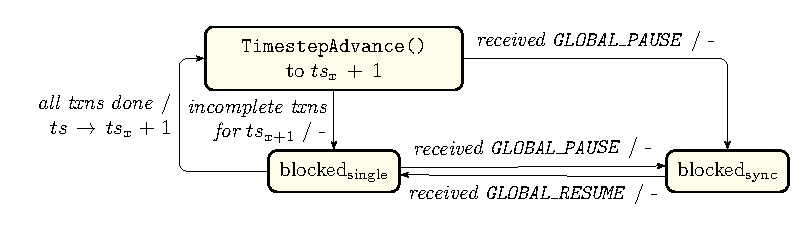
\includegraphics[keepaspectratio]{../tikz-exps/pdf/mpistate.pdf}}

}

\caption{TimestepAdvance State Transitions}

\end{figure}%
\end{frame}

\begin{frame}{Current Status}
\phantomsection\label{current-status}
\begin{itemize}
\tightlist
\item
  Aggregation overlay exists

  \begin{itemize}
  \tightlist
  \item
    Overlay supports mutiple aggregators, SQL only on single
  \end{itemize}
\end{itemize}

\pause

\begin{itemize}
\tightlist
\item
  MPI-side interfaces for schemas and probes exists
\end{itemize}

\pause

\begin{itemize}
\tightlist
\item
  Core TS2PC infra exists

  \begin{itemize}
  \tightlist
  \item
    TS2PC for probes exists
  \item
    TS2PC for dynamic queries: TODO
  \item
    TS2PC for online tuning: TODO
  \end{itemize}
\end{itemize}

\pause

\begin{itemize}
\tightlist
\item
  TUI exists
\end{itemize}

\pause

\begin{itemize}
\tightlist
\item
  Immediate next steps:

  \begin{itemize}
  \tightlist
  \item
    How to visualize telemetry?
  \item
    Option 1: export slice to trace
  \item
    Option 2: real-time views
  \end{itemize}
\end{itemize}

\pause

\begin{itemize}
\tightlist
\item
  After: distributed queries
\end{itemize}
\end{frame}

\begin{frame}{Realtime Views: Challenge and Ideas}
\phantomsection\label{realtime-views-challenge-and-ideas}
\begin{itemize}
\tightlist
\item
  We have a highly programmable observability system
\item
  Visualization is a function of current query
\end{itemize}

\pause

\begin{itemize}
\tightlist
\item
  Persisting telemetry via Parquet: implemented-ish

  \begin{itemize}
  \tightlist
  \item
    Can be used for offline analysis
  \end{itemize}
\end{itemize}

\pause

\begin{itemize}
\tightlist
\item
  Unclear how to incorporate a Grafana-like frontend

  \begin{itemize}
  \tightlist
  \item
    Grafana does not understand timesteps
  \item
    Supports plugins, thinking about how to write one
  \end{itemize}
\end{itemize}
\end{frame}

\begin{frame}[fragile]{Misc: Substrait for SQL}
\phantomsection\label{misc-substrait-for-sql}
\begin{itemize}
\tightlist
\item
  Substrait: (emerging) intermediate representation for SQL
\item
  Advantage: may not need Datafusion/Rust on most nodes
\end{itemize}

\pause

\begin{itemize}
\tightlist
\item
  Apache Acero: execution engine in \texttt{arrow-cpp}

  \begin{itemize}
  \tightlist
  \item
    Given an Arrow table + Substrait plan, can execute
  \end{itemize}
\end{itemize}

\pause

\begin{itemize}
\tightlist
\item
  Still need datafusion for distributed query planning

  \begin{itemize}
  \tightlist
  \item
    (At a head node or something) . . .
  \end{itemize}
\item
  May have teething issues
\end{itemize}

\pause

\begin{figure}[H]

{\centering \pandocbounded{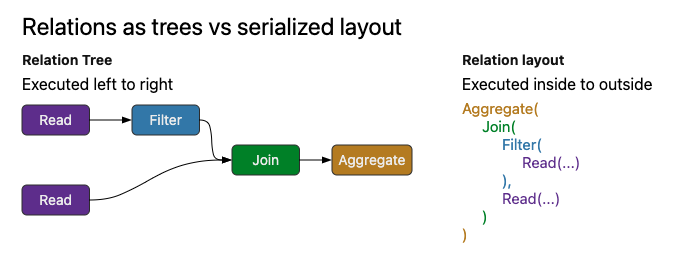
\includegraphics[keepaspectratio]{images/substrait.png}}

}

\caption{Substrait for SQL}

\end{figure}%
\end{frame}




\end{document}
